\section{Systemarchitektur}\label{sec:systemarchitektur}

Es gibt 3 große Services, das Chat Widget auf der Schulhompage, das Dashboard und das Backend.
Unser System sieht folgendermaßen aus:

\begin{figure}[hbt!]
    \centering
    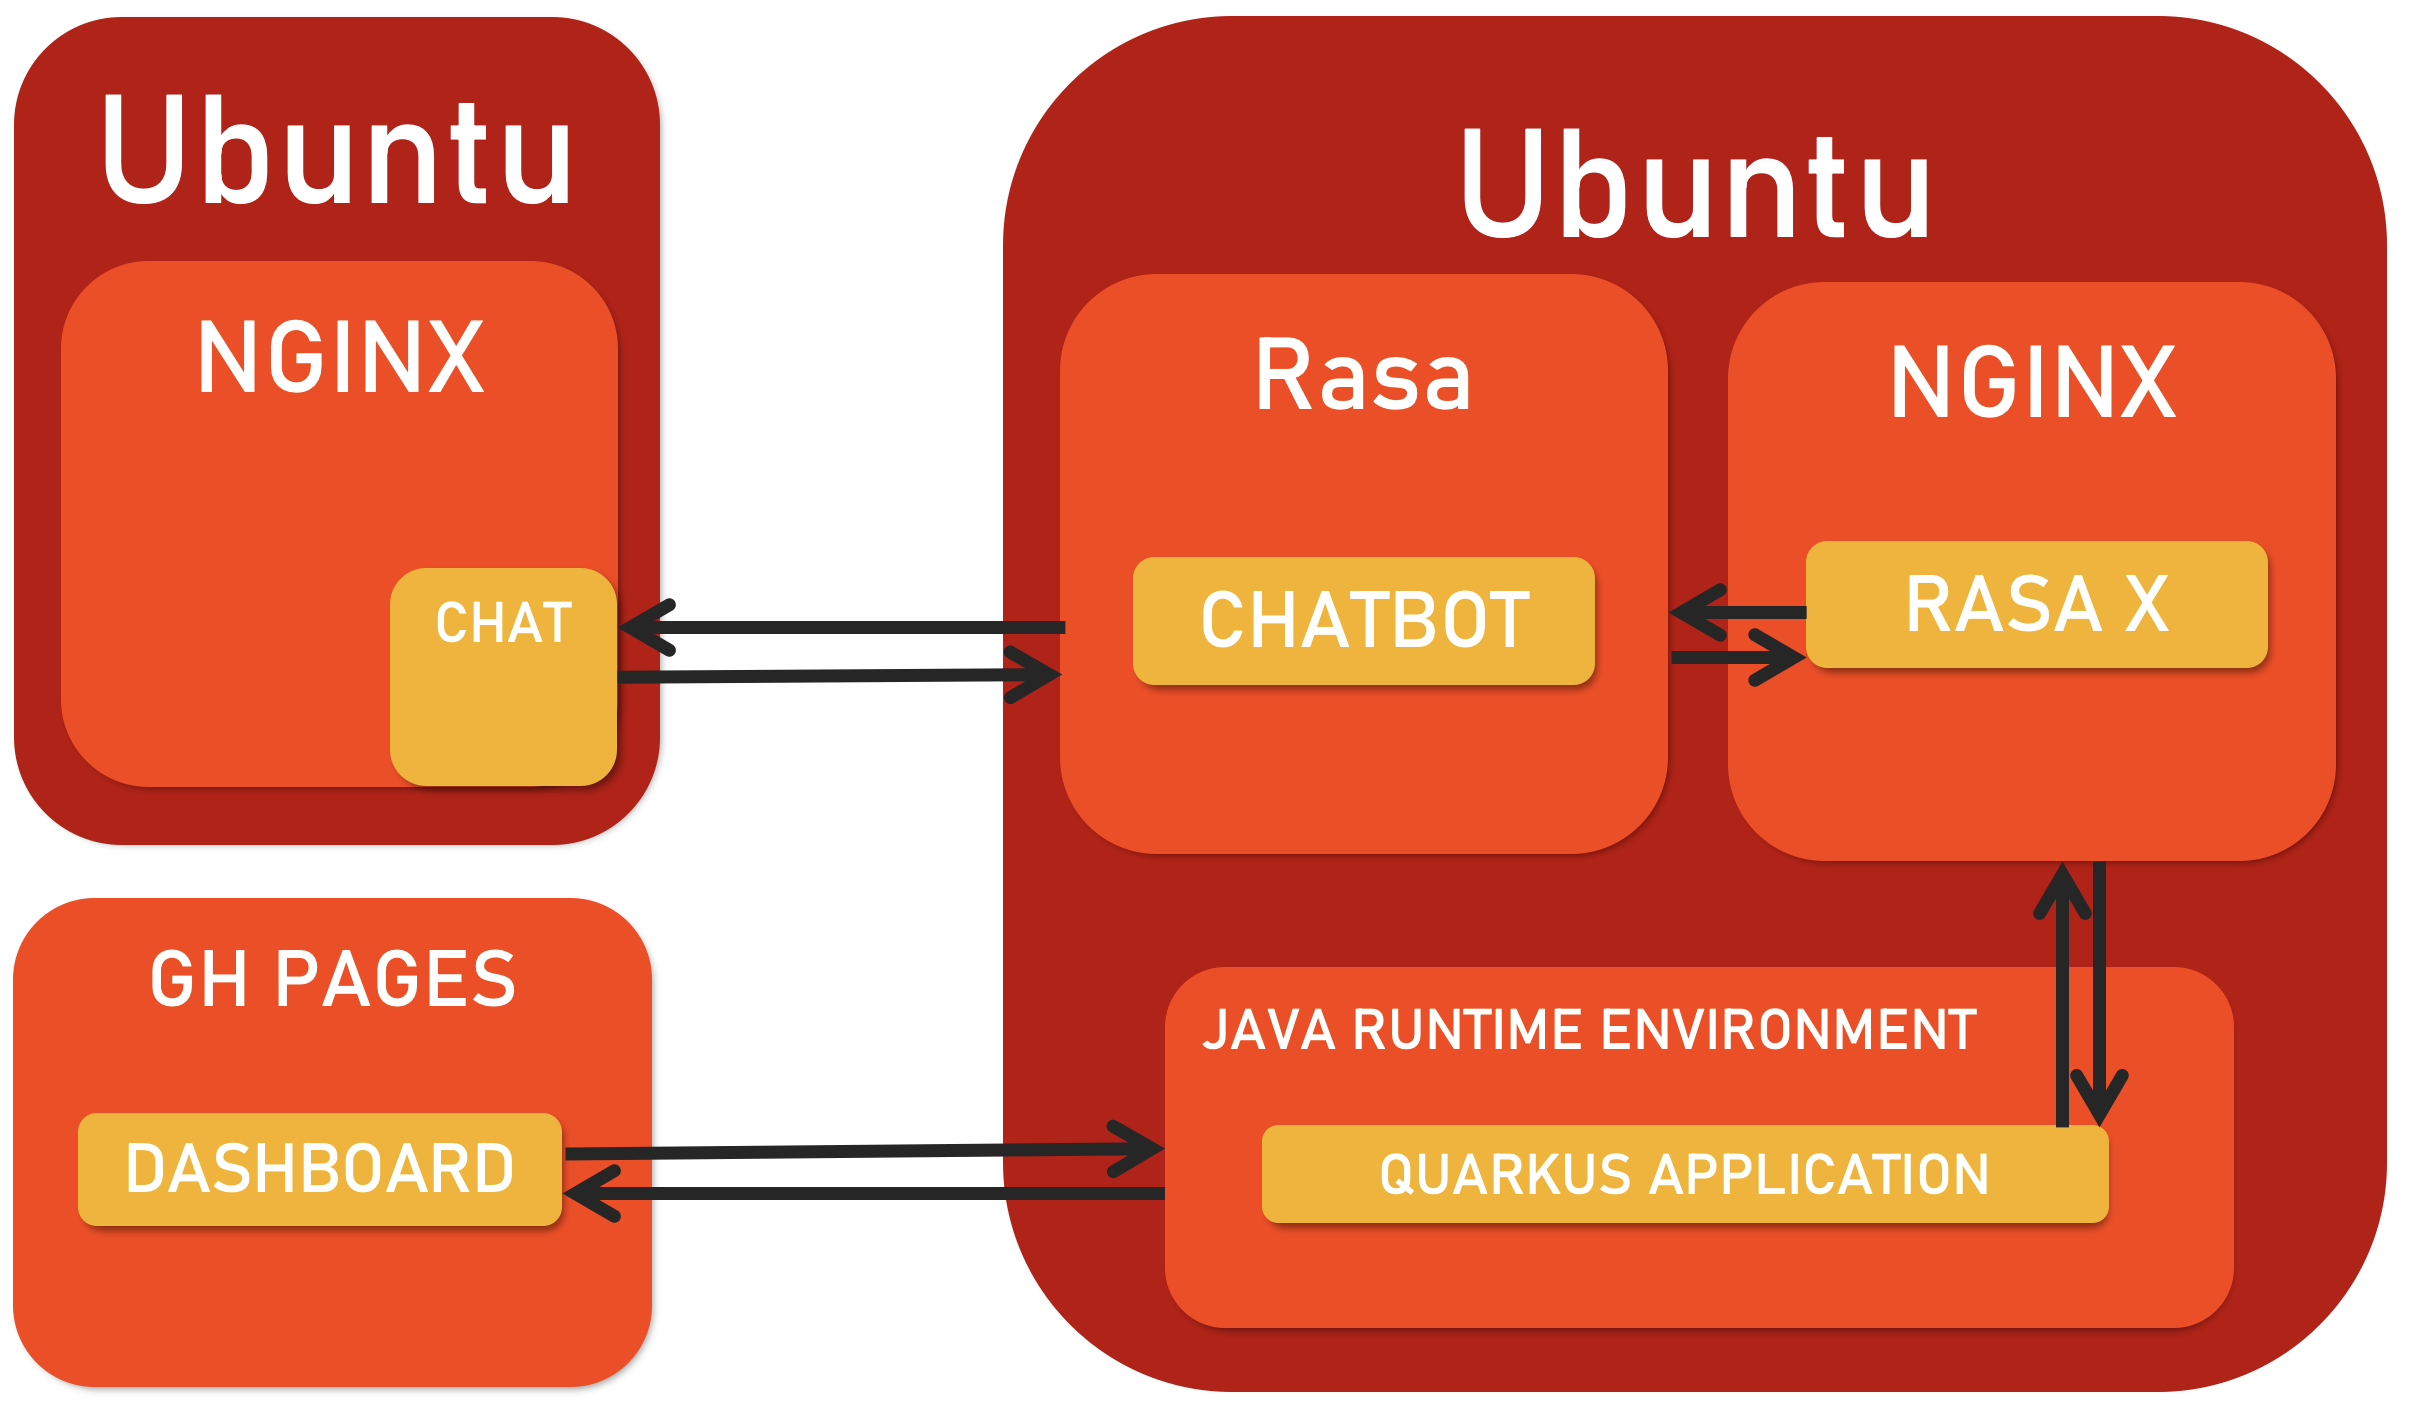
\includegraphics[scale=0.2]{pics/systemarchitektur}
    \caption{Systemarchitektur}
    \label{fig:impl:architektur}
\end{figure}

Wir haben 2 Ubuntu VM's, eine für den Chat und eine für Rasa und das Backend, nachdem der Chat auf die HTL Leonding Seite kommt, wird dadurch nur noch eine VM benötigt.

Unser Chat wird gerade mit NGINX gehostet, dieser kommuniziert mit Rasa direkt über REST, wenn der Benutzer eine Nachricht sendet, wird diese an Rasa gesendet und Rasa antwortet mit der passenden Antwort.
Das Dashboard wird auf GH Pages gehostet, dieses kommuniziert mit dem Backend über REST, das Backend authentisiert sich bei Rasa X\ref{subsec:rasa-x} und holt sich alle Konversationen und bereitet diese auf und sendet sie an das Dashboard.

\section{Backend}\label{sec:backend}
\setauthor{Felix Dumfarth}

Unser Quarkus ~\ref{quarkus} Backend hat die Aufgabe mit Rasa X zu kommunizieren und die Konversationsdaten für das Dashboard aufzubereiten und zu senden.

Unser Backend besitzt folgende Endpoints:

\begin{itemize}
    \item GET /api/conversations
    \item GET /api/conversations/{id}
    \item POST /api/feedback
    \item GET /api/feedback
    \item GET /api/file/{filename}
    \item PUT /api/file/{filename}
\end{itemize}

Bei den beiden ``conversations'' endpoints muss man sich aber zuerst authentisieren und sich einen Bearer Token von Rasa x holen damit man auf die anderen Rasa X endpoints zugreifen kann .

\subsection{GET /api/conversations}
Der Endpoint ruft zuerst die getAuth() funktion auf, um den Bearer Token zu erhalten.

Danach wird der Rasa X GET Endpoint /api/conversations aufgerufen mit dem Bearer Token im Header.
Von diesem Endpoint wird ein JSON Objekt zurückgegeben, das die Konversationen enthält, aber zusätzlich noch viele andere unrelevante Daten, deshalb holt sich das Backend wirklich nur ID des Senders, die Zeit und die Anzahl von Nachrichten der Unterhaltungen.

\subsection{GET /api/conversations/{id}}
Der Endpoint /api/conversations/{id} ruft zuerst die getAuth() funktion auf, um den Bearer Token zu erhalten.

Um nur von einer gezielten Unterhaltung die Nachrichten zu erhalten wird der Rasa X Endpint /api/conversations/{id}/messages aufgerufen mit dem Bearer Token im Header.
Die Response wird auch in dieser Form schon zurückgeben, da die Response keine unwichtigen Daten enthält.

\subsection{POST /api/feedback}
Der Endpoint /api/feedback erhält ein JSON Objekt mit den Daten des Feedback Formulars und speichert diese in die Datenbank.

\subsection{GET /api/feedback}
Der Endpoint /api/feedback liest alle Feedbacks aus der Datenbank und gibt diese zurück.

\subsection{GET /api/file/{filename}}
Der Endpoint /api/file/{filename} liest die im URL angegeben Datei aus dem Filesystem aus und gibt diese zurück.
Die möglichen Dateinamen sind:

\begin{itemize}
    \item nlu.yml
    \item rules.yml
    \item stories.yml
    \item config.yml
    \item domain.yml
\end{itemize}

\subsection{PUT /api/file/{filename}}
Der Endpoint /api/file/{filename} erhält den Inhalt aus dem File welches auch im URL angegeben wurde und überschreibt dieses dann im Filesystem.

\section{Chat Widget}\label{sec:chat-widget}
Der Chatbot der HTL Leonding sollte auf der Schulhomepage als Chatblase angezeigt werden, und verschiedene Elemente wie Buttons und Links unterstzützen.

\subsection{Konzept}
Während den Anfängen der vorliegenden Arbeit wurde ein Konzept erstellt, um das mögliche Aussehen festzulegen. Lange Zeit wurde der Chatbot unter den Namen Leon geführt.
Dies wurde jedoch im späteren verlauf geändert und Leon wurde Teil des langjährigen Leonie Projektes der HTL Leonding.
Ursprünglich war das Symbol des Chatbots, wie man am Konzept sehen kann, ein Bot. Durch den wechsel in die Leonie Familie wurde dieses Logo jedoch gegen Leonie getauscht.
\begin{figure}[hbt!]
    \centering
    \includegraphics[scale=0.2]{pics/conceptBotClosed.png}
    \caption{Konzept Chatbot geschlossen}
    \label{fig:impl:conceptBotClosed}
\end{figure}
\begin{figure}[hbt!]
    \centering
    \includegraphics[scale=0.2]{pics/conceptBotOpen.png}
    \caption{Konzept Chatbot geöffnet}
    \label{fig:impl:conceptBotOpen}
\end{figure}

\subsection{Umsetzung}
Umgesetzt wurde das Frontend mithilfe von Angular. Die Chatblase ist eine eigene Komponente, die durch CSS immer rechts unten fixiert ist. Die Farben des Chatbots sollten natürlich an die HTL Leonding erinnern, deshalb wurde ein Farbverlauf aus Farben des HTL Logos erstellt.

Jedoch begann der Chatbot sehr anders, zu begin wurde der Bot zuerst als ganze Seite entwickelt und nicht nur als Chatblase.
\begin{figure}[hbt!]
    \centering
    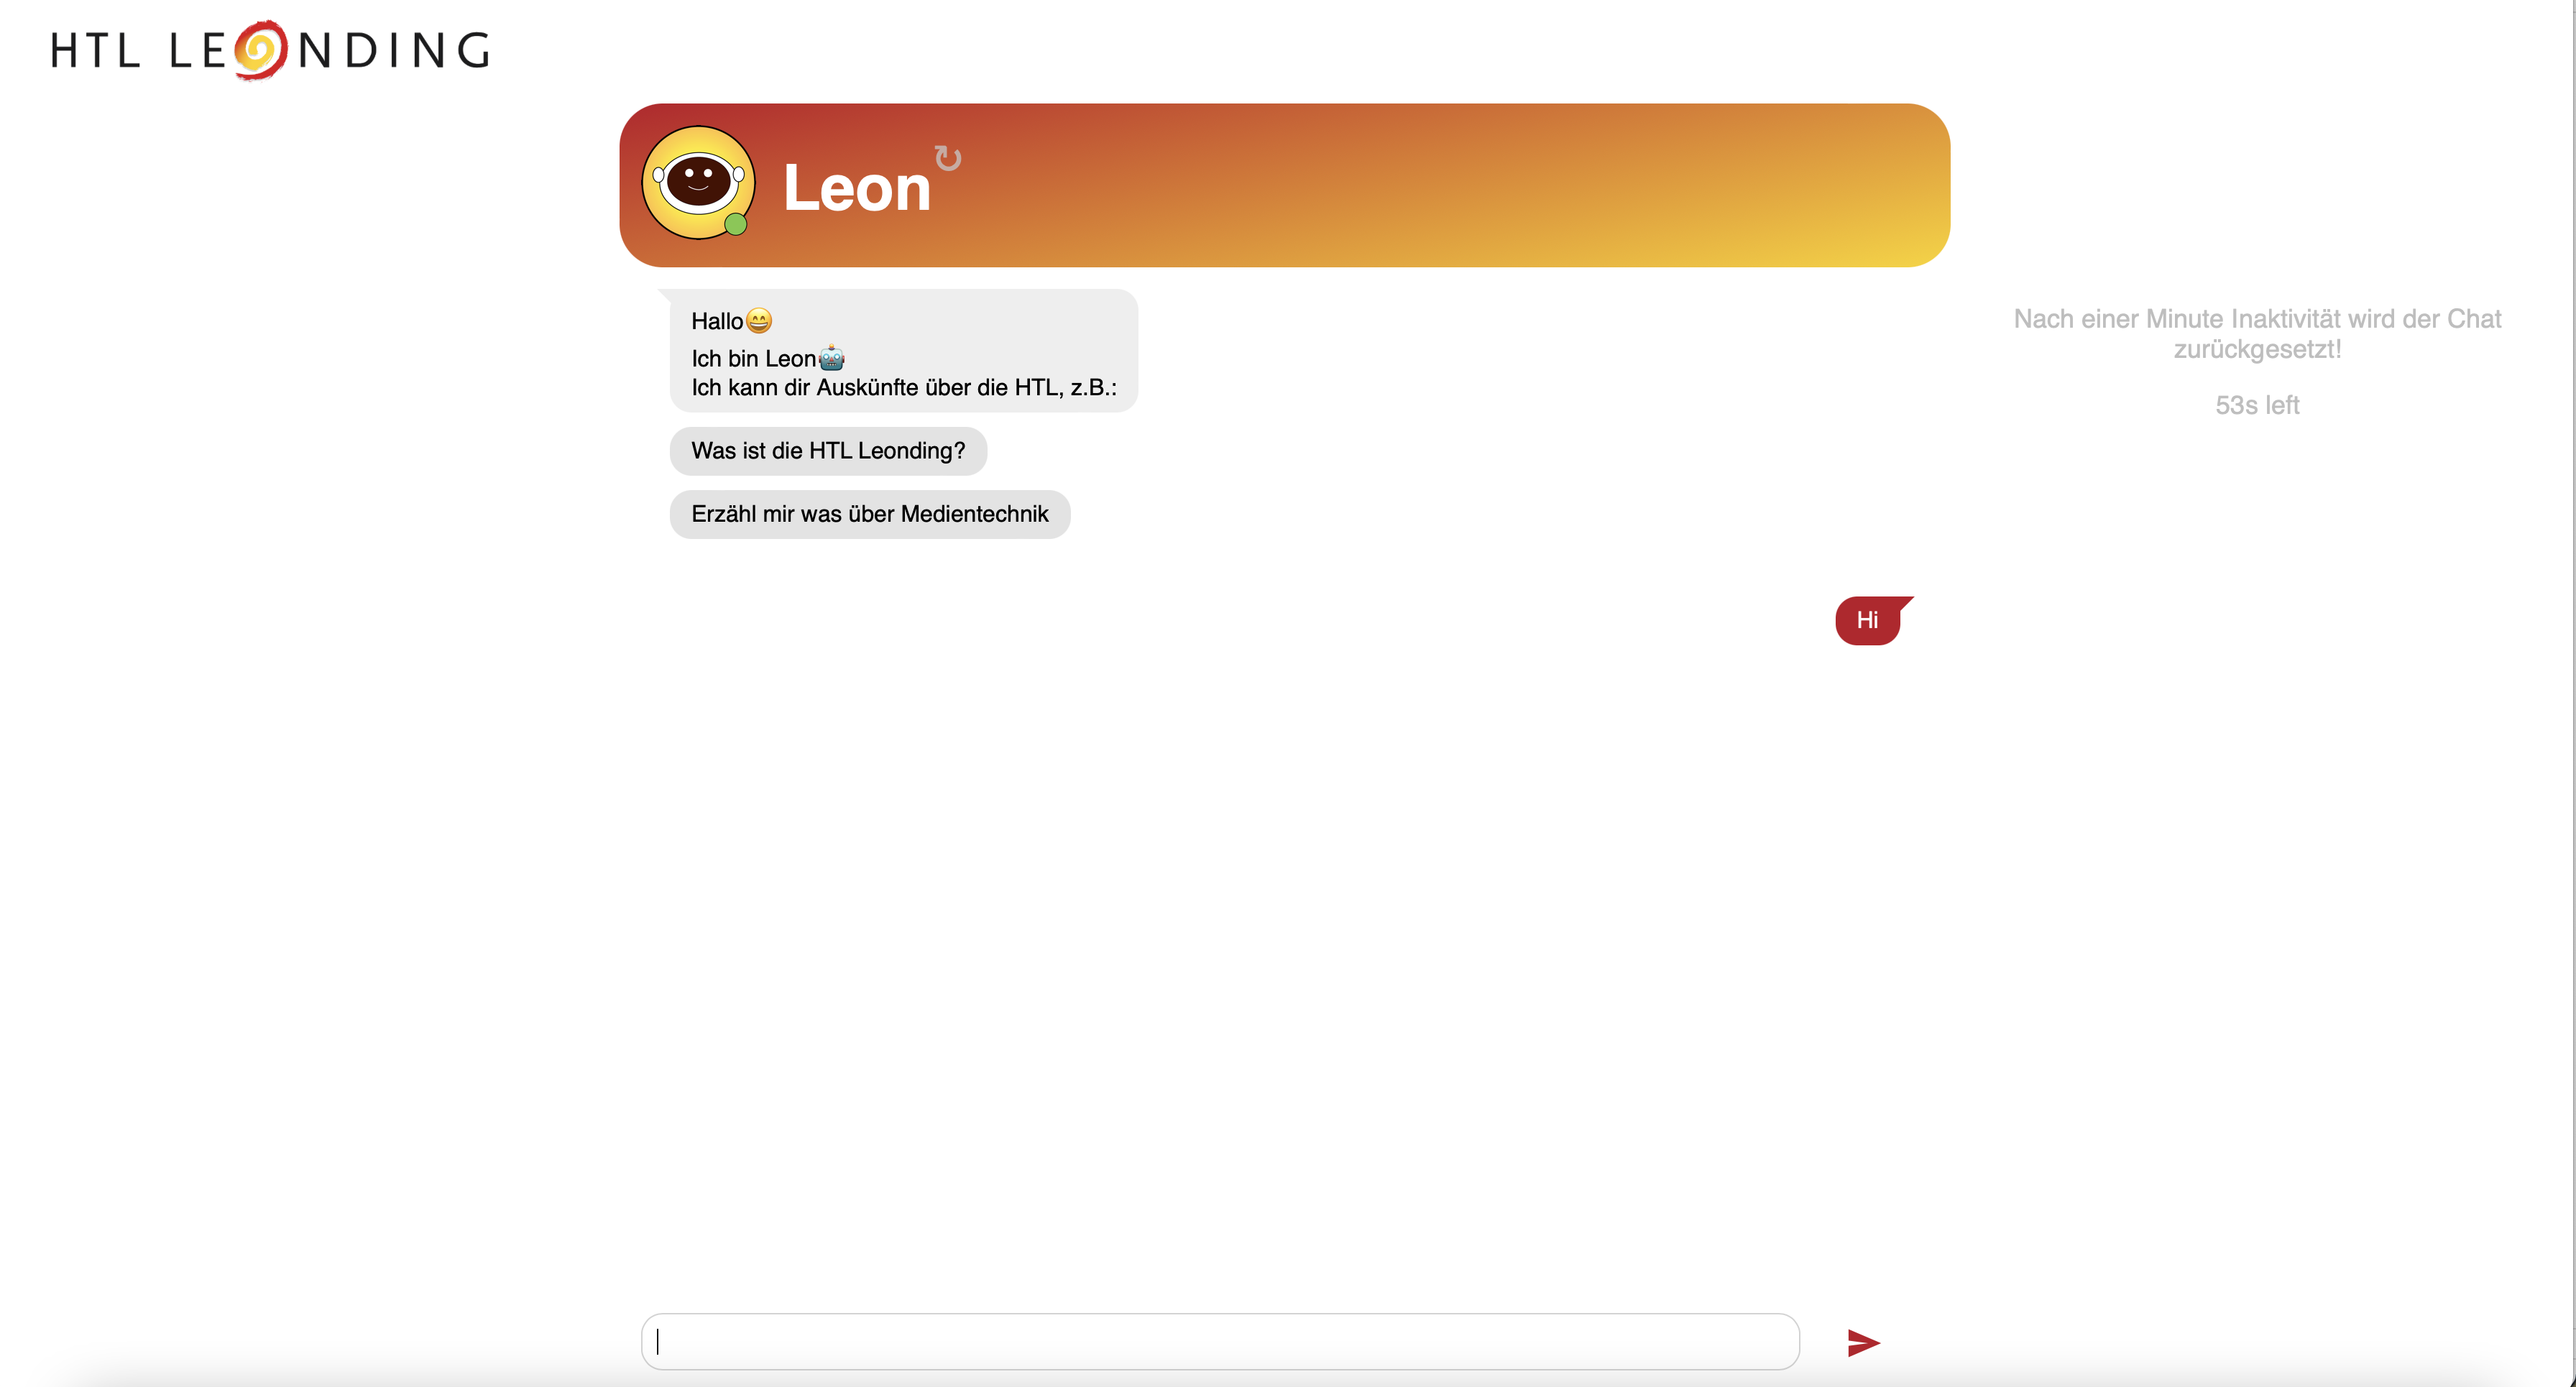
\includegraphics[scale=0.2]{pics/fullPageBot.png}
    \caption{Chatbot auf einer ganzen Seite}
    \label{fig:impl:conceptBotFullPage}
\end{figure}

Natürlich war dies nicht das endgültige Ziel so wurde der Bot schnell zur Chatblase umgewandelt.
Zum Testen war die HTL Leonding Seite mithilfe eines IFrames eingebunden und zusätzlich die Chatblasen Komponente.

Um das Gespräch in eine Richtung zu lenken wurden Buttons eingeführt, die nach fast jeder Antwort mögliche folge Fragen vorschlagen.

\begin{figure}[hbt!]
    \centering
    \includegraphics[scale=0.2]{pics/finalBot.png}
    \caption{Chatbot}
    \label{fig:impl:bot}
\end{figure}

Um Bewertungen von echten Benutzern zu holen wurde außerdem eine Feedback Seite eingeführt, in dieser kann der Benutzer eine 1 bis 5 Sterne bewertung und einen Text absenden.

%TODO: Bilder zum Feedback


Die Chatblase wurde in einem eigenen Modul entwickelt, um die Komponenten zu verstecken und zu verbergen.

Das Chatfenster wurde in 3 Bereiche geteilt.

\begin{figure}[hbt!]
    \centering
    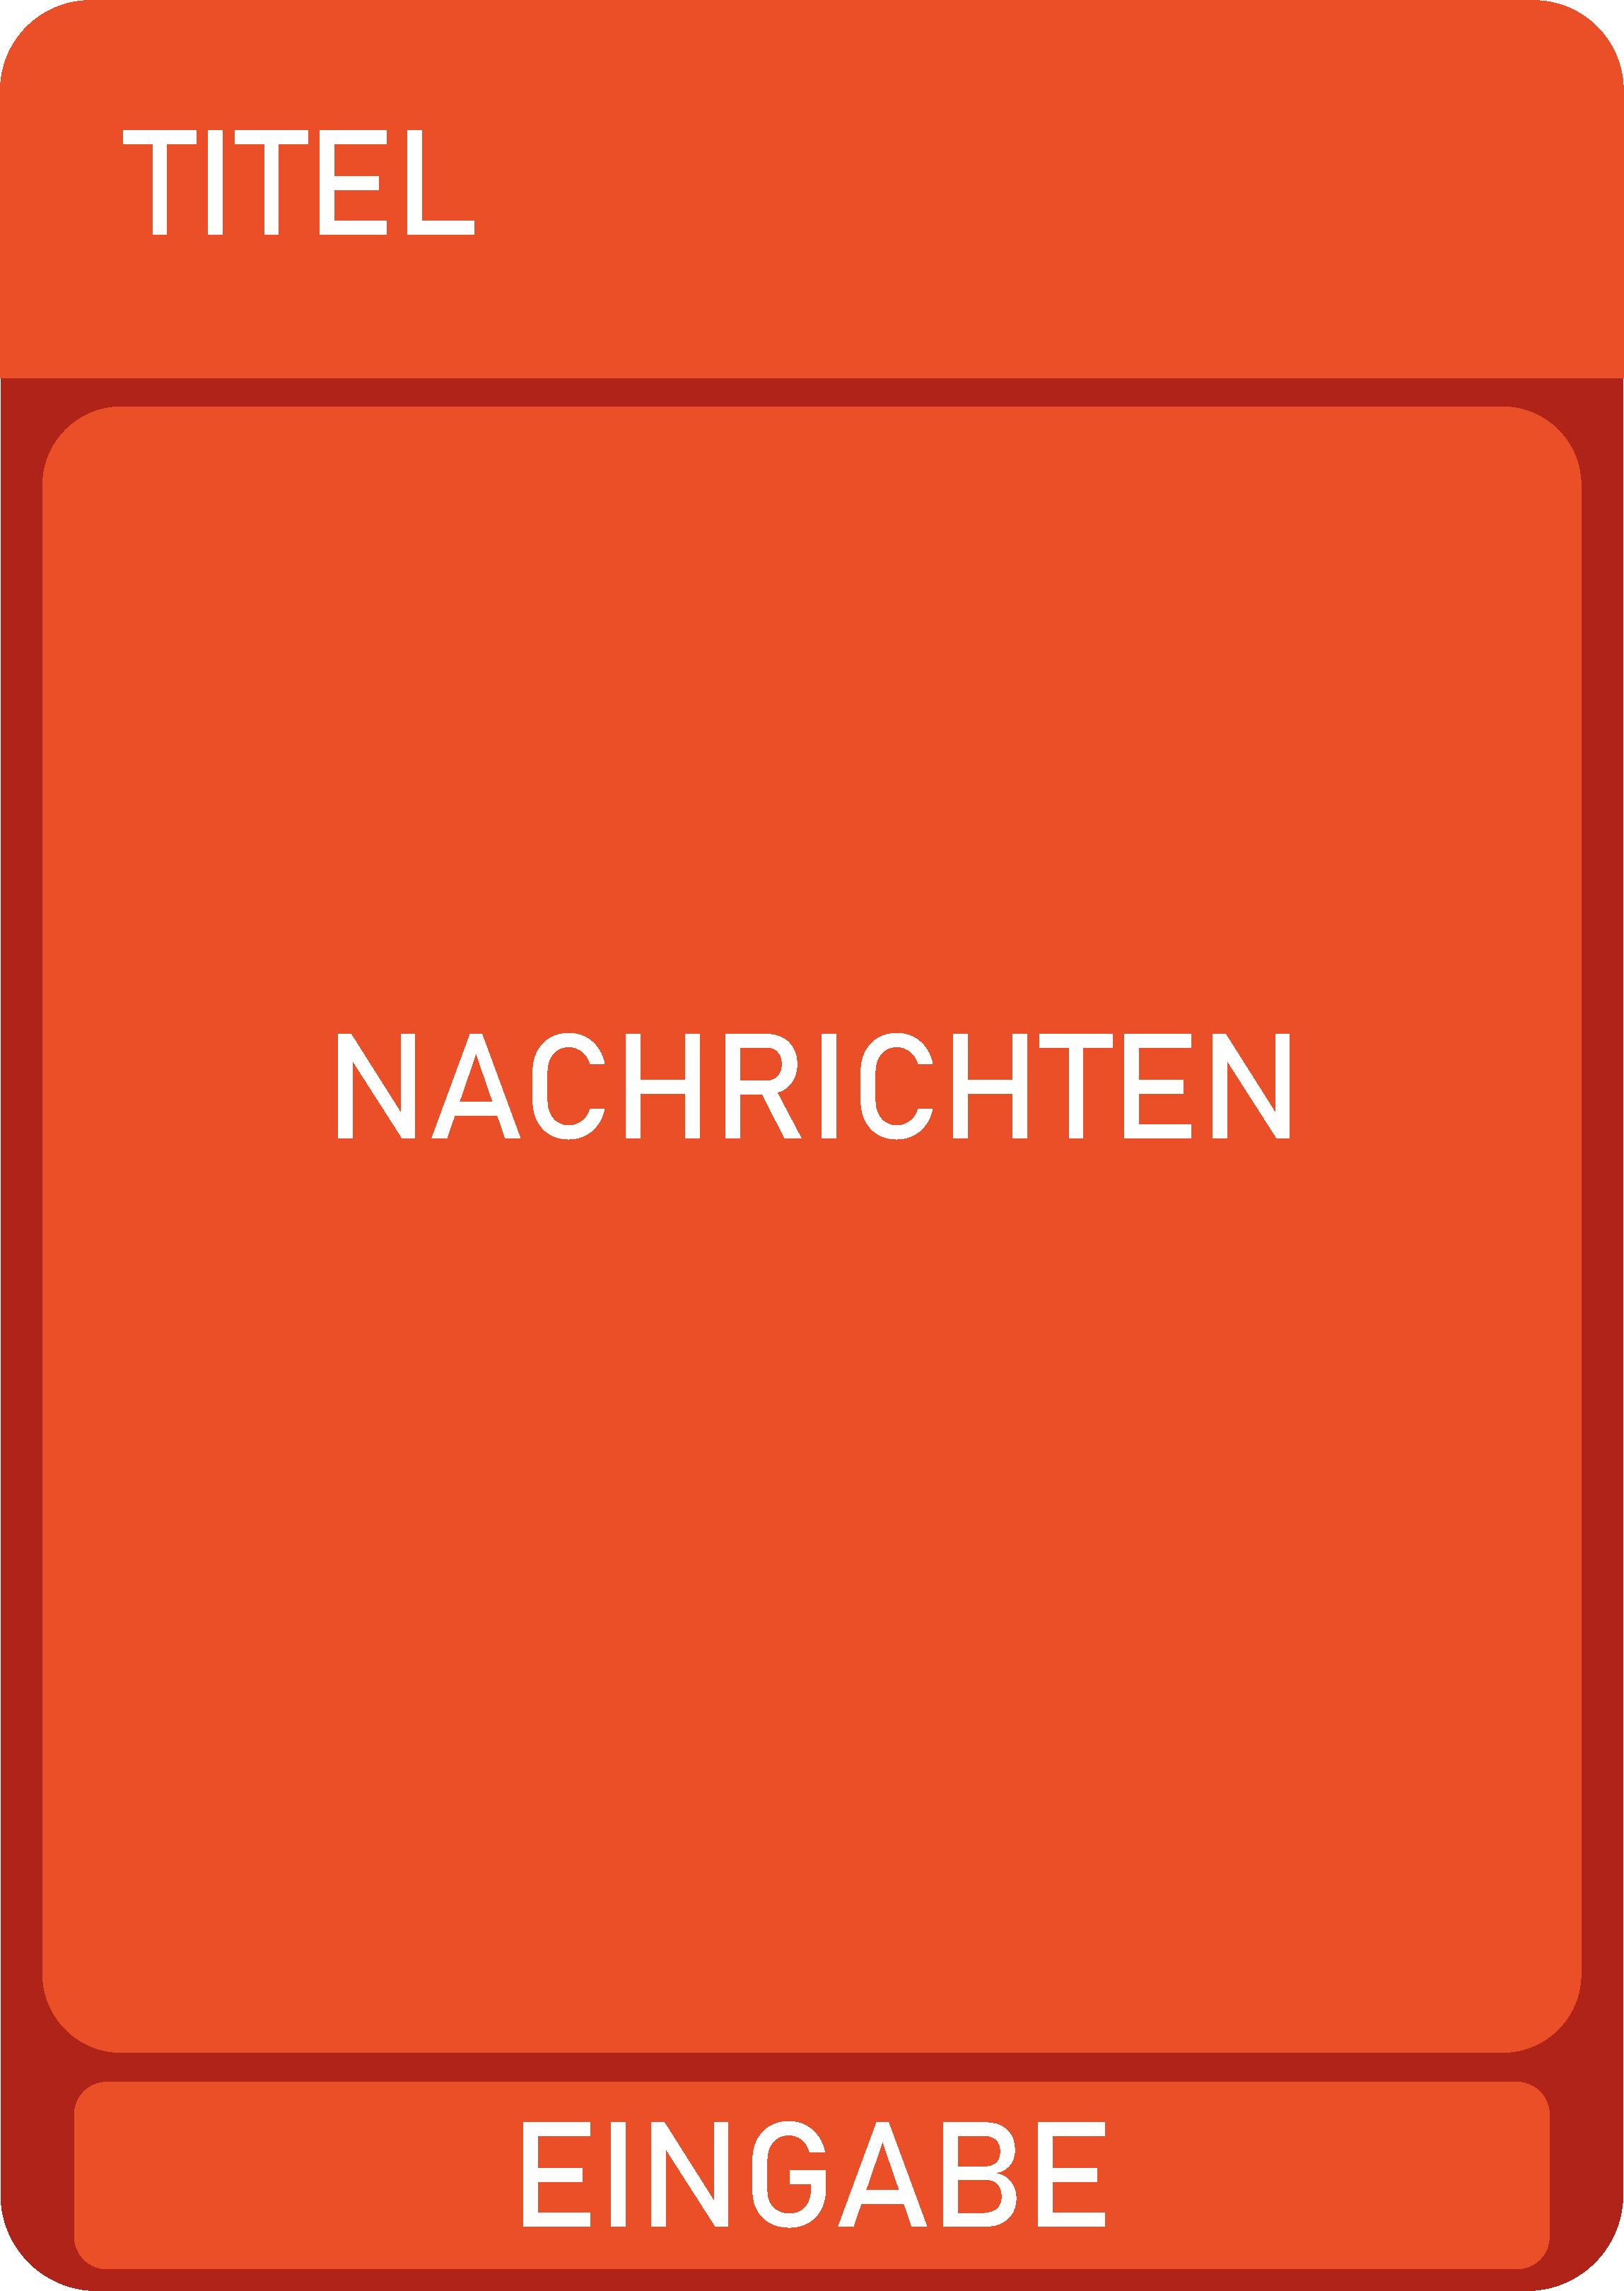
\includegraphics[scale=0.2]{pics/chatWidgetStructure}
    \caption{Aufbau vom Chat Fenster}
    \label{fig:impl:chatWidget}
\end{figure}


\section{Dashboard}\label{sec:dashboard}

Um alle Gespräche und die Bewertungen der Benutzer anzuzeigen wurde ein Dashboard eingeführt, wo nur dies möglich war.
Im Laufe der Arbeit wurde dieses dann erweitert, um für den Leobot Conversation Cycle als Seite zu dienen.

\subsection{Conversation-Driven Development}\label{cdd}
Rasa empfiehlt für die Entwicklung von Chatbots ``Conversation-Driven Development'', kurz CDD.\cite{cdd}
Aber was ist CDD?

CDD beschreibt eine Entwicklungsstrategie, in der du deinen Chatbot nach Konversationen mit echten Usern verbesserst.

Bei CDD wird empfohlen, dass man seinen Chatbot möglichst früh echten Benutzern zur verfügung stehlt und so beobachten kann was die echten Benutzer alles für Intents erwarten und wie sie ihre Anfragen formulieren und kann diese bei Bedarf hinzufügen.



\subsection{Leobot Conversation Cycle}

\begin{figure}[hbt!]
    \centering
    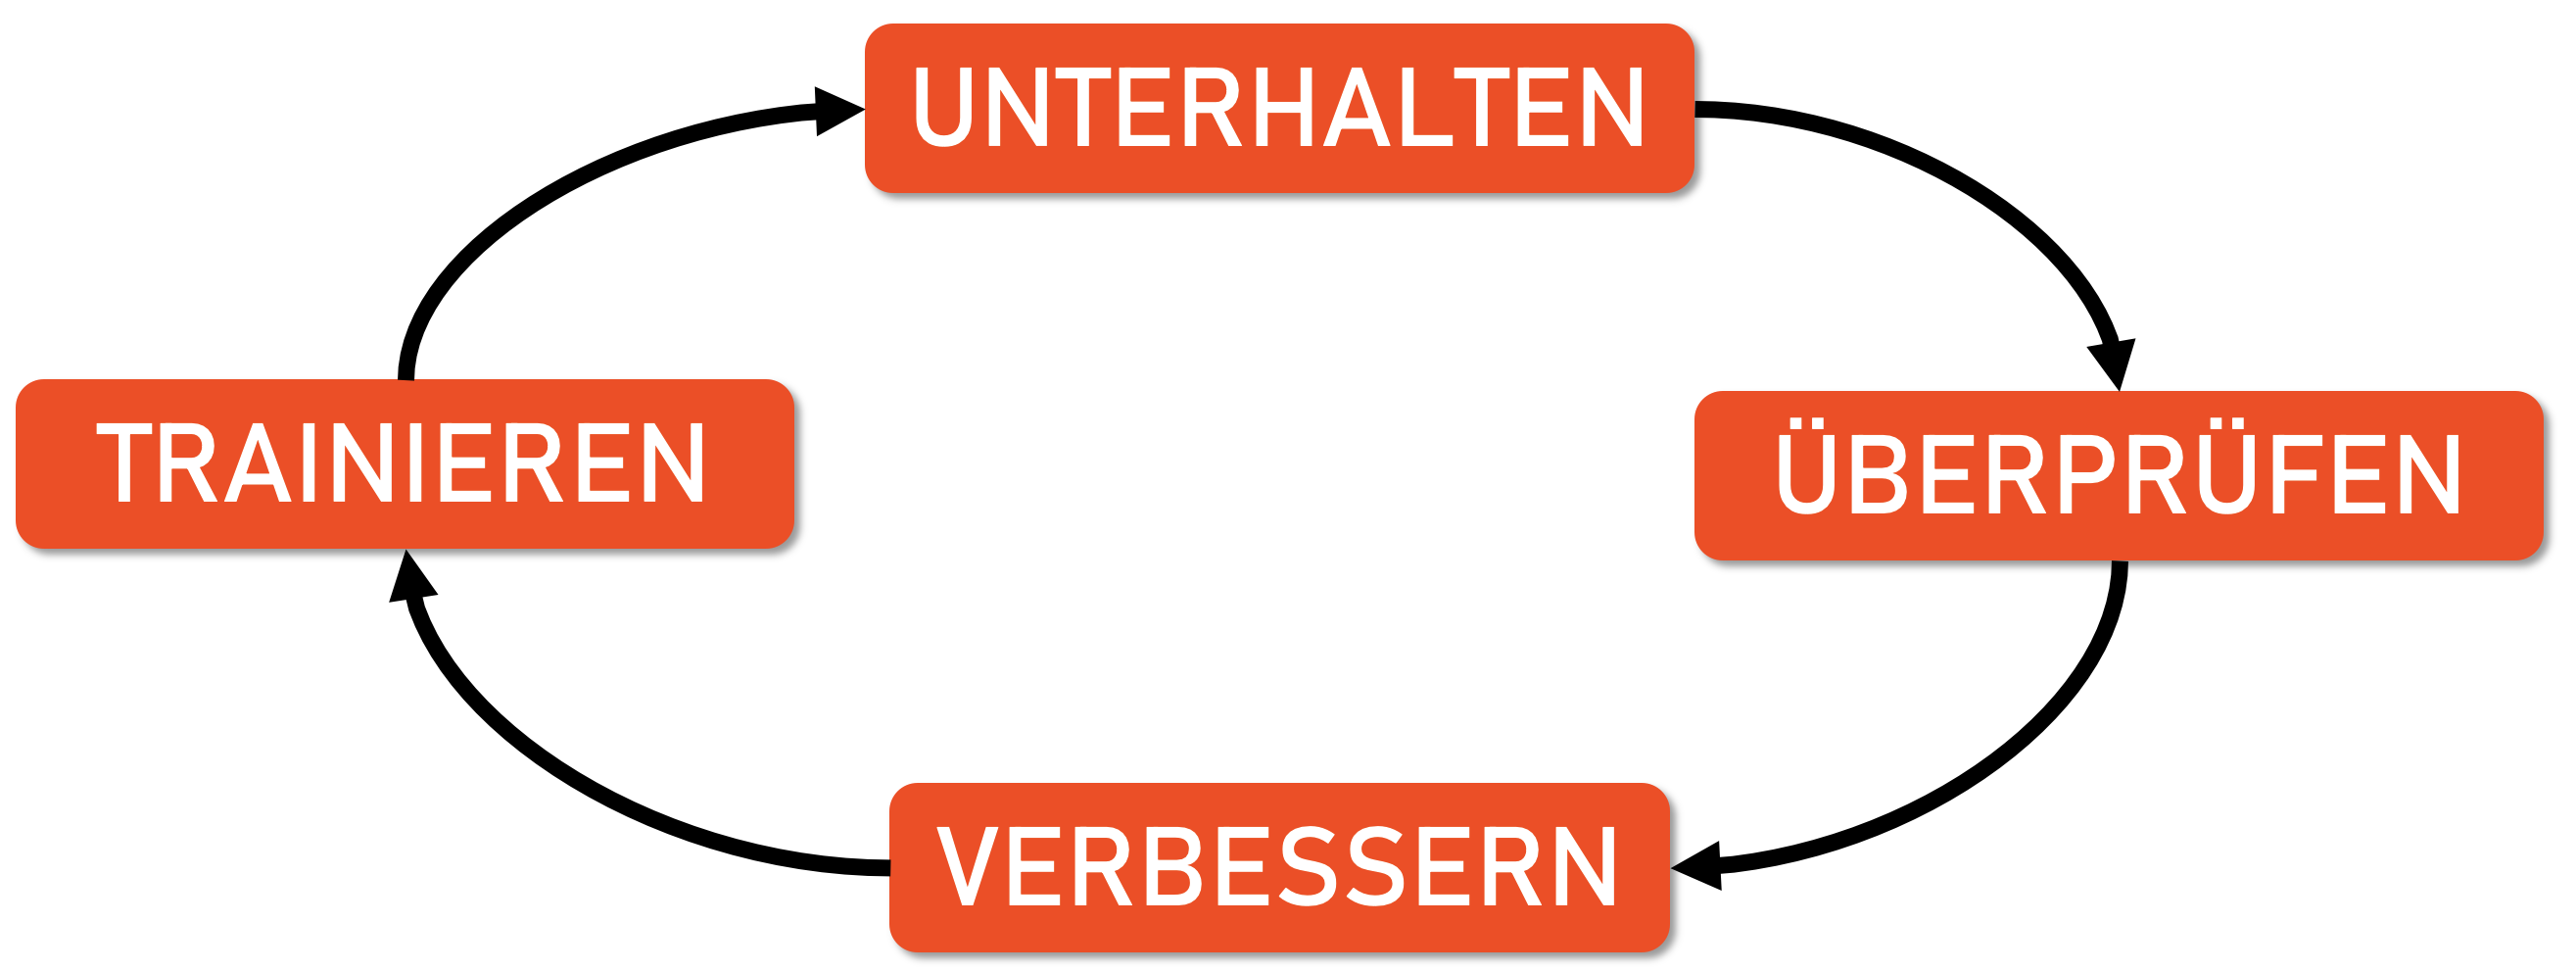
\includegraphics[scale=0.2]{pics/LeoCircle}
    \caption{Leobot Conversation Cycle}
    \label{fig:impl:ConversationCycle}
\end{figure}

Wir setzen CDD ~\ref{cdd} mithilfe unsres Leobot Conversation Cycle um, der Leobot Conversation Cycle ist ein Workflow, der dazu dient, den Leobot zu überprüfen und zu erweitern.

Der Workflow besteht aus folgenden Schritten:

\begin{itemize}
    \item Unterhalten
    \item Überprüfen
    \item Verbessern
    \item Trainieren
\end{itemize}

Diese 4 Schritte werden immer wieder durchgeführt um den Chatbot dauerhaft zu verbessern.

\subsubsection{Unterhalten}
Unterhalten ist der erste Schritt des Leobot Conversation Cycles, in diesem Schritt werden dem Bot Fragen gestellt, die er beantworten muss, dies passiert natürlich während Unterhaltungen im Chat auf der Schulhompage.
Die Unterhaltungen werden dann alle gespeichert.

\subsubsection{Überprüfen}
Überprüfen ist der zweite Schritt des Leobot Conversation Cycles, in diesem Schritt wird der Bot überprüft, ob er die Fragen richtig beantwortet und erkannt hat.
Dieser Schritt wird von Verantwortlichen für den Leobot durchgeführt.

\subsubsection{Verbessern}
Verbessern ist der dritte Schritt des Leobot Conversation Cycles, in diesem Schritt wird der Bot verbessert, das heißt die Fehler werden versucht zu beheben.
Je nachdem was der fehler des Bots war muss hier anders gearbeitet werden.
Wenn er einen Intent den er eigentlich kennt aber die Formulierung des Benutzers so war das er diesen nicht erkannt hat, wird die Eingabe des Benutzers zu den Trainingsdaten hinzugefügt.

Falls jemand aber eine Frage stellt zu der es keinen Intent gibt und sich die Verantwortlichen denken es wäre ein guter Intent so wird der ganze Intent zu den Trainingsdaten hinzugefügt.

\subsubsection{Trainieren}
Trainieren ist der vierte Schritt des Leobot Conversation Cycles, in diesem Schritt werden die Trainingsdaten an den Bot übergeben und dieser Trainiert und wechselt auf das neu trainierte Model.

Und nun beginnt der Leobot Conversation Cycle wieder von vorne.

\subsection{Umsetzung}

Einerseits kann man sich die vergangenen Unterhaltungen ansehen, so wie die nlu.yml, stories.yml, rules.yml, domain.yml direkt im Monaco Editor bearbeiten und speichern.

\begin{figure}[hbt!]
    \centering
    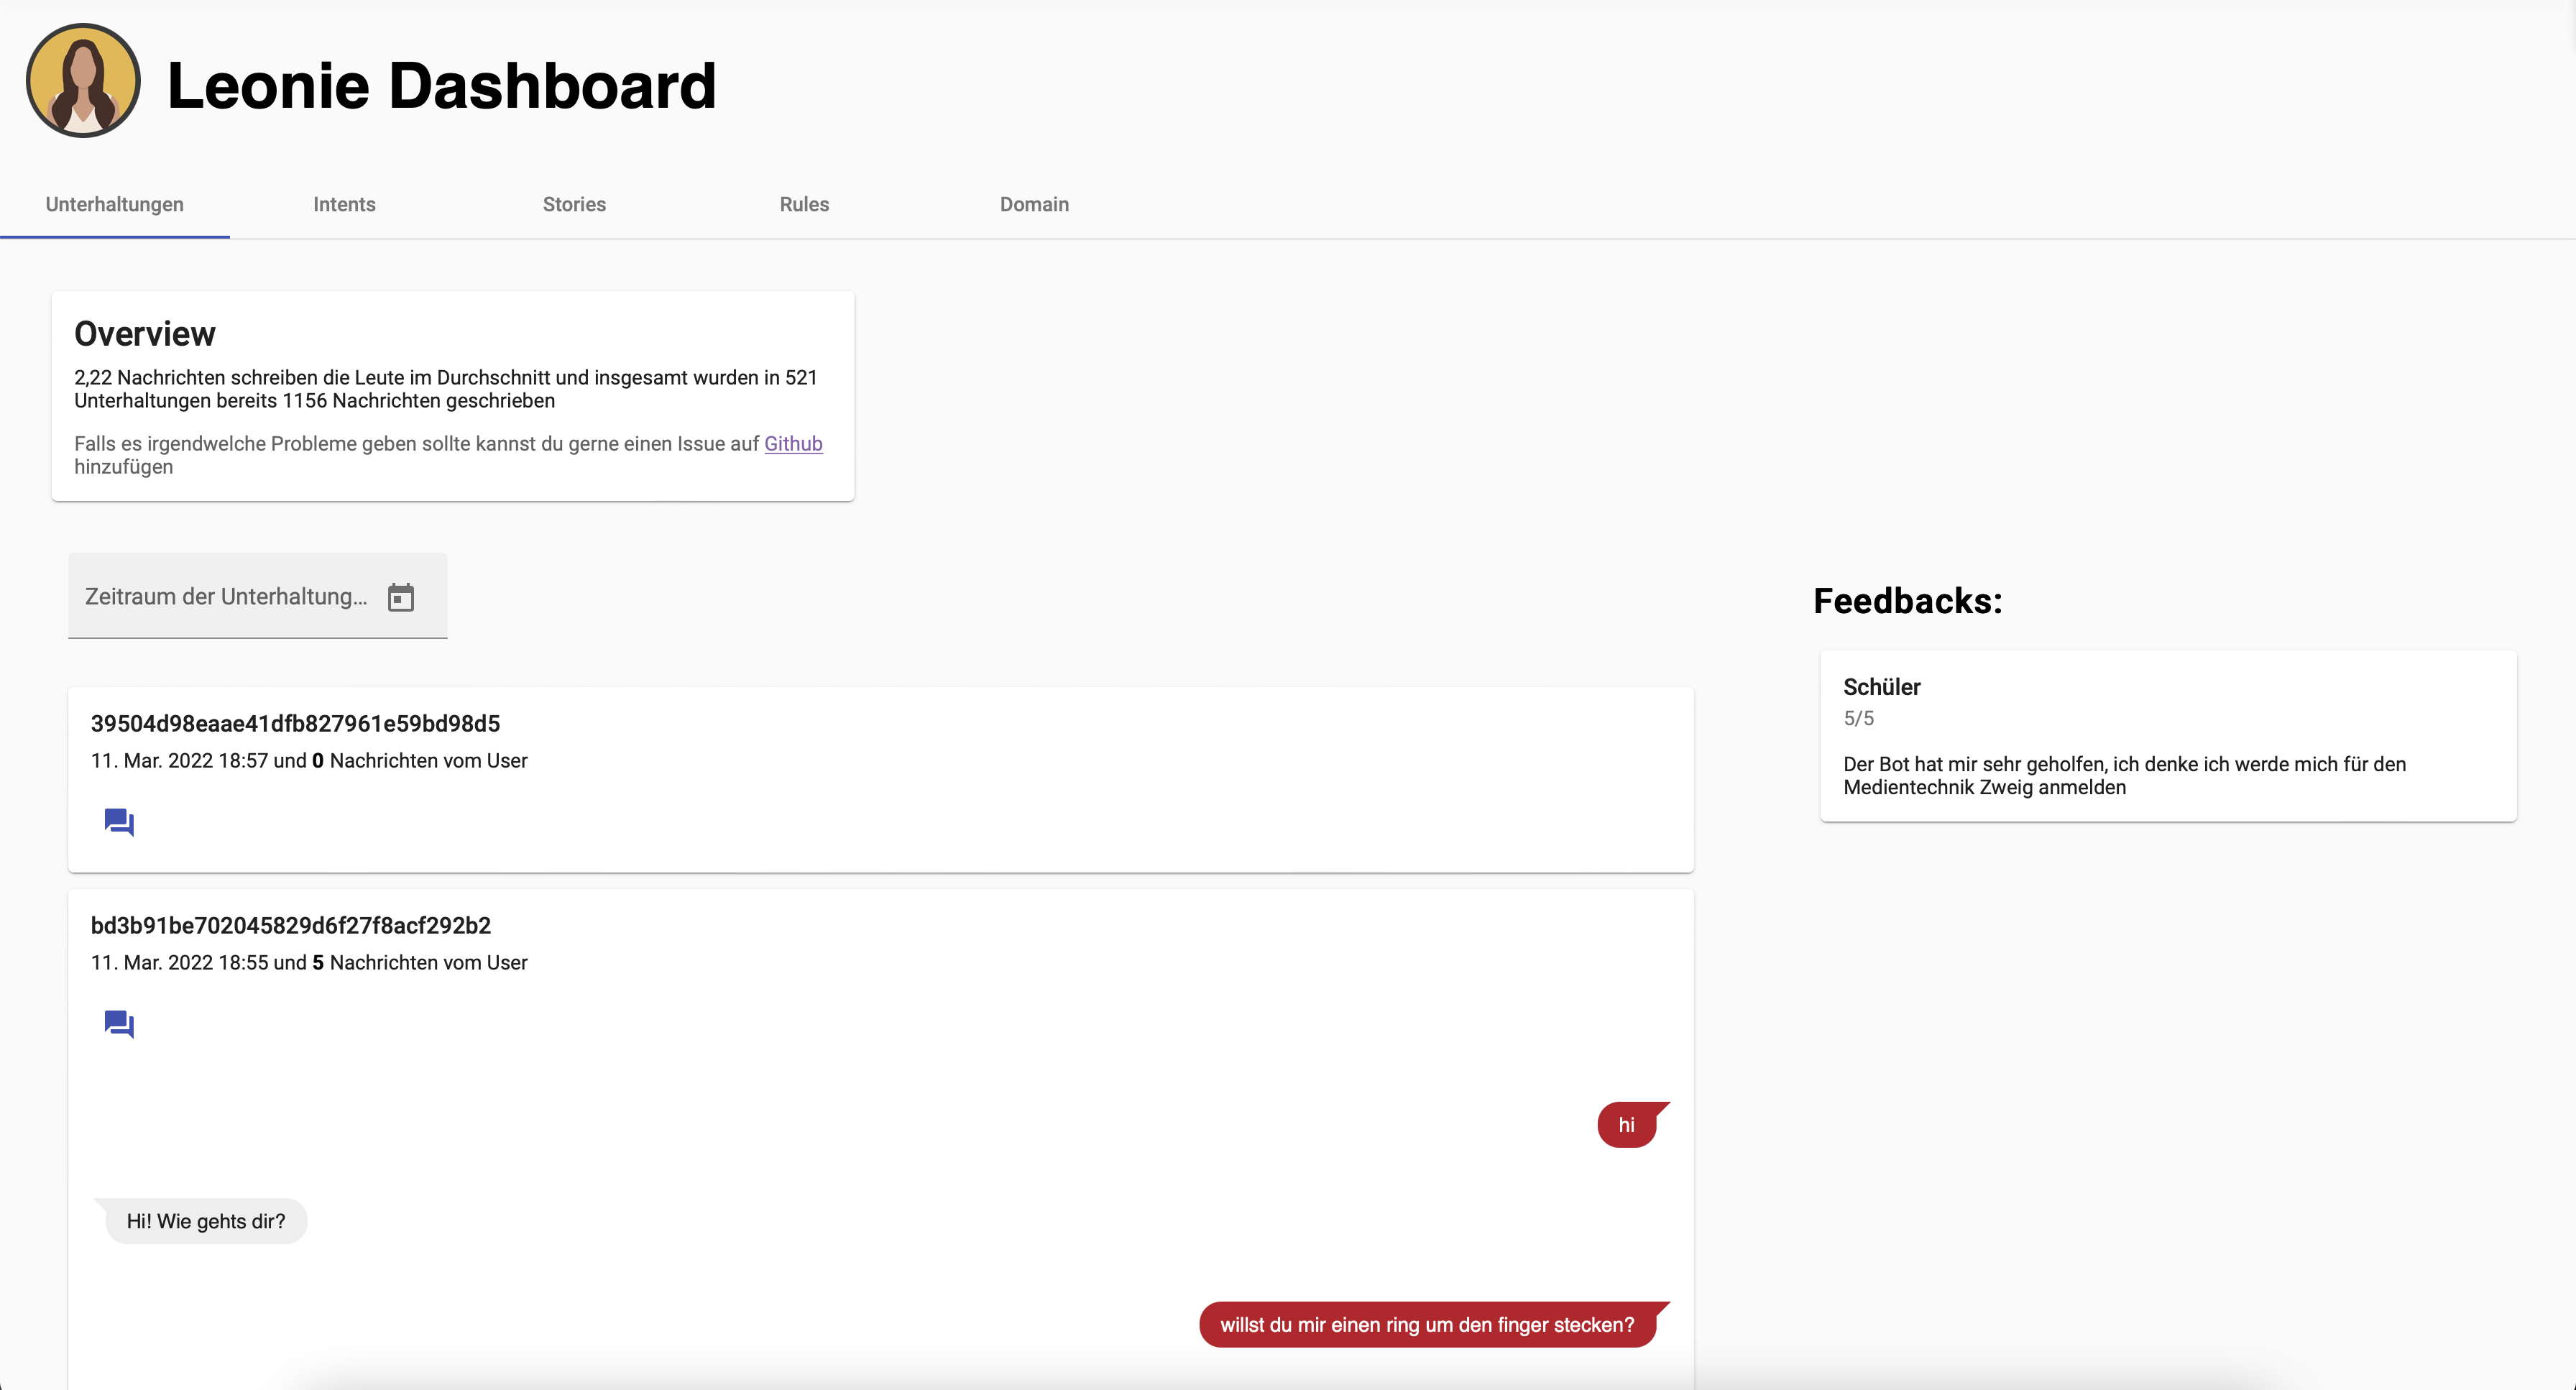
\includegraphics[scale=0.2]{pics/dashboardConvo}
    \caption{Dashboard}
    \label{fig:impl:dashConv}
\end{figure}

Im Editor wurden auch Code Vorschläge benutzt um etwas an Tipparbeit sparen zu können.

\begin{figure}[hbt!]
    \centering
    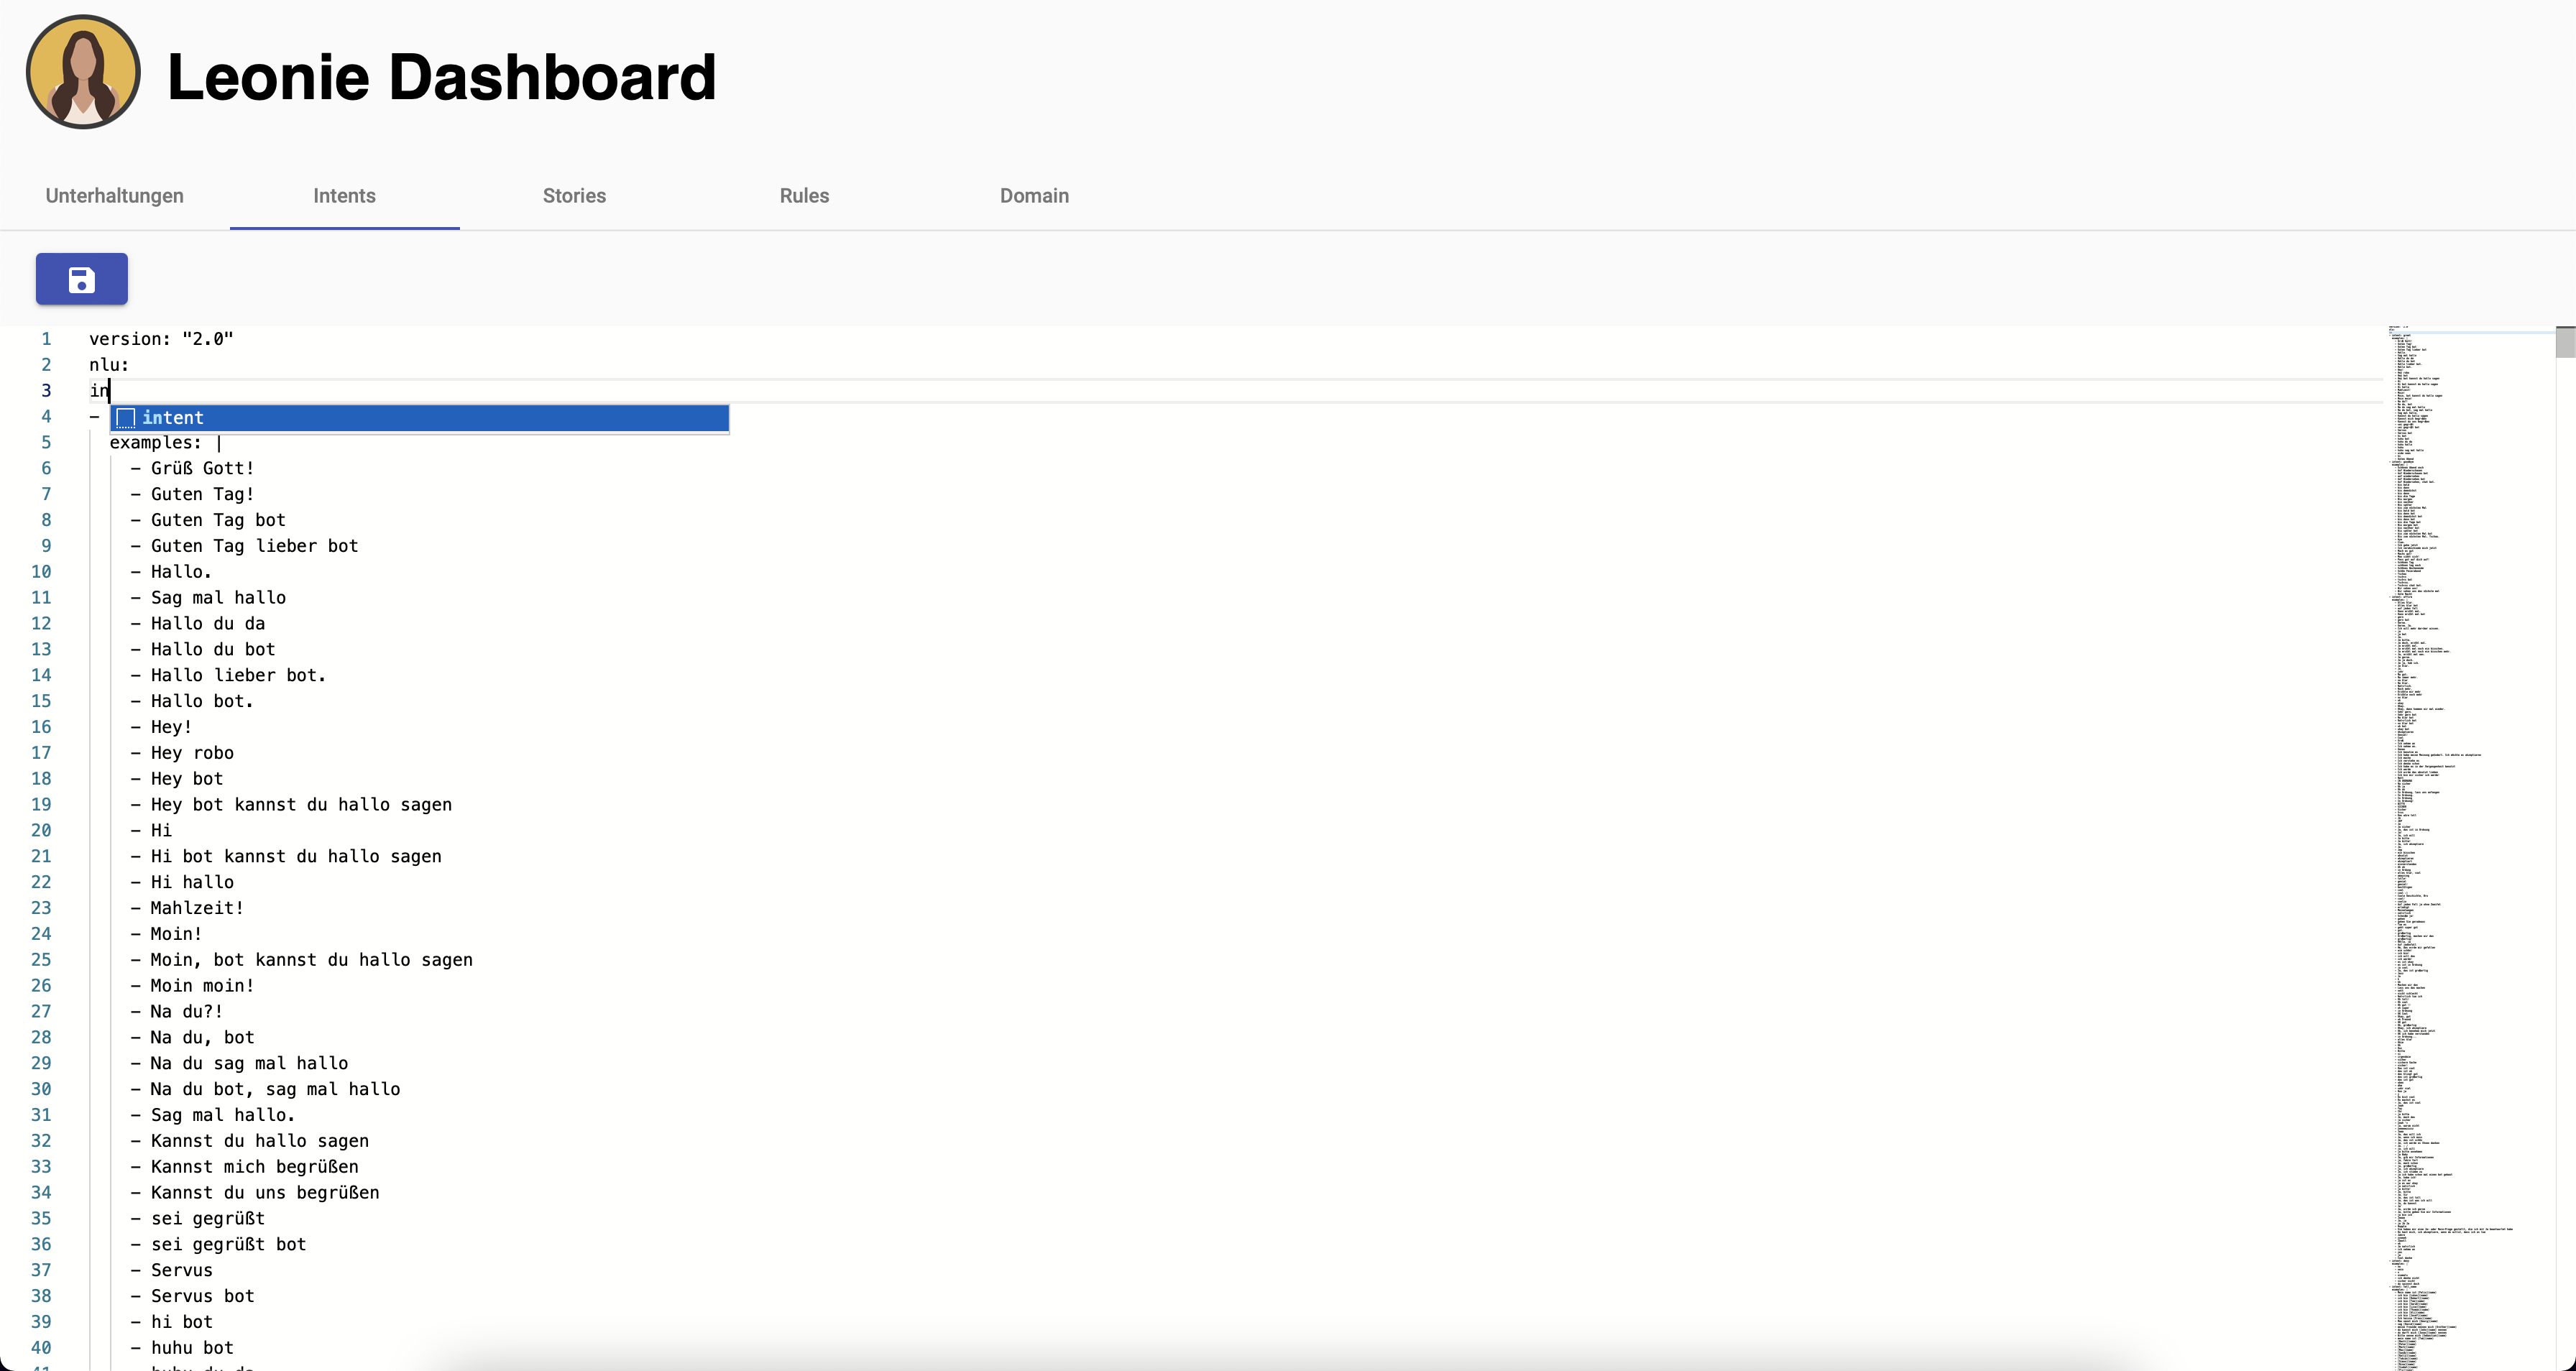
\includegraphics[scale=0.2]{pics/dashboardCodeSuggestion}
    \caption{Vorschläge}
    \label{fig:impl:dashboardCodeSuggestion}
\end{figure}
\begin{figure}[hbt!]
    \centering
    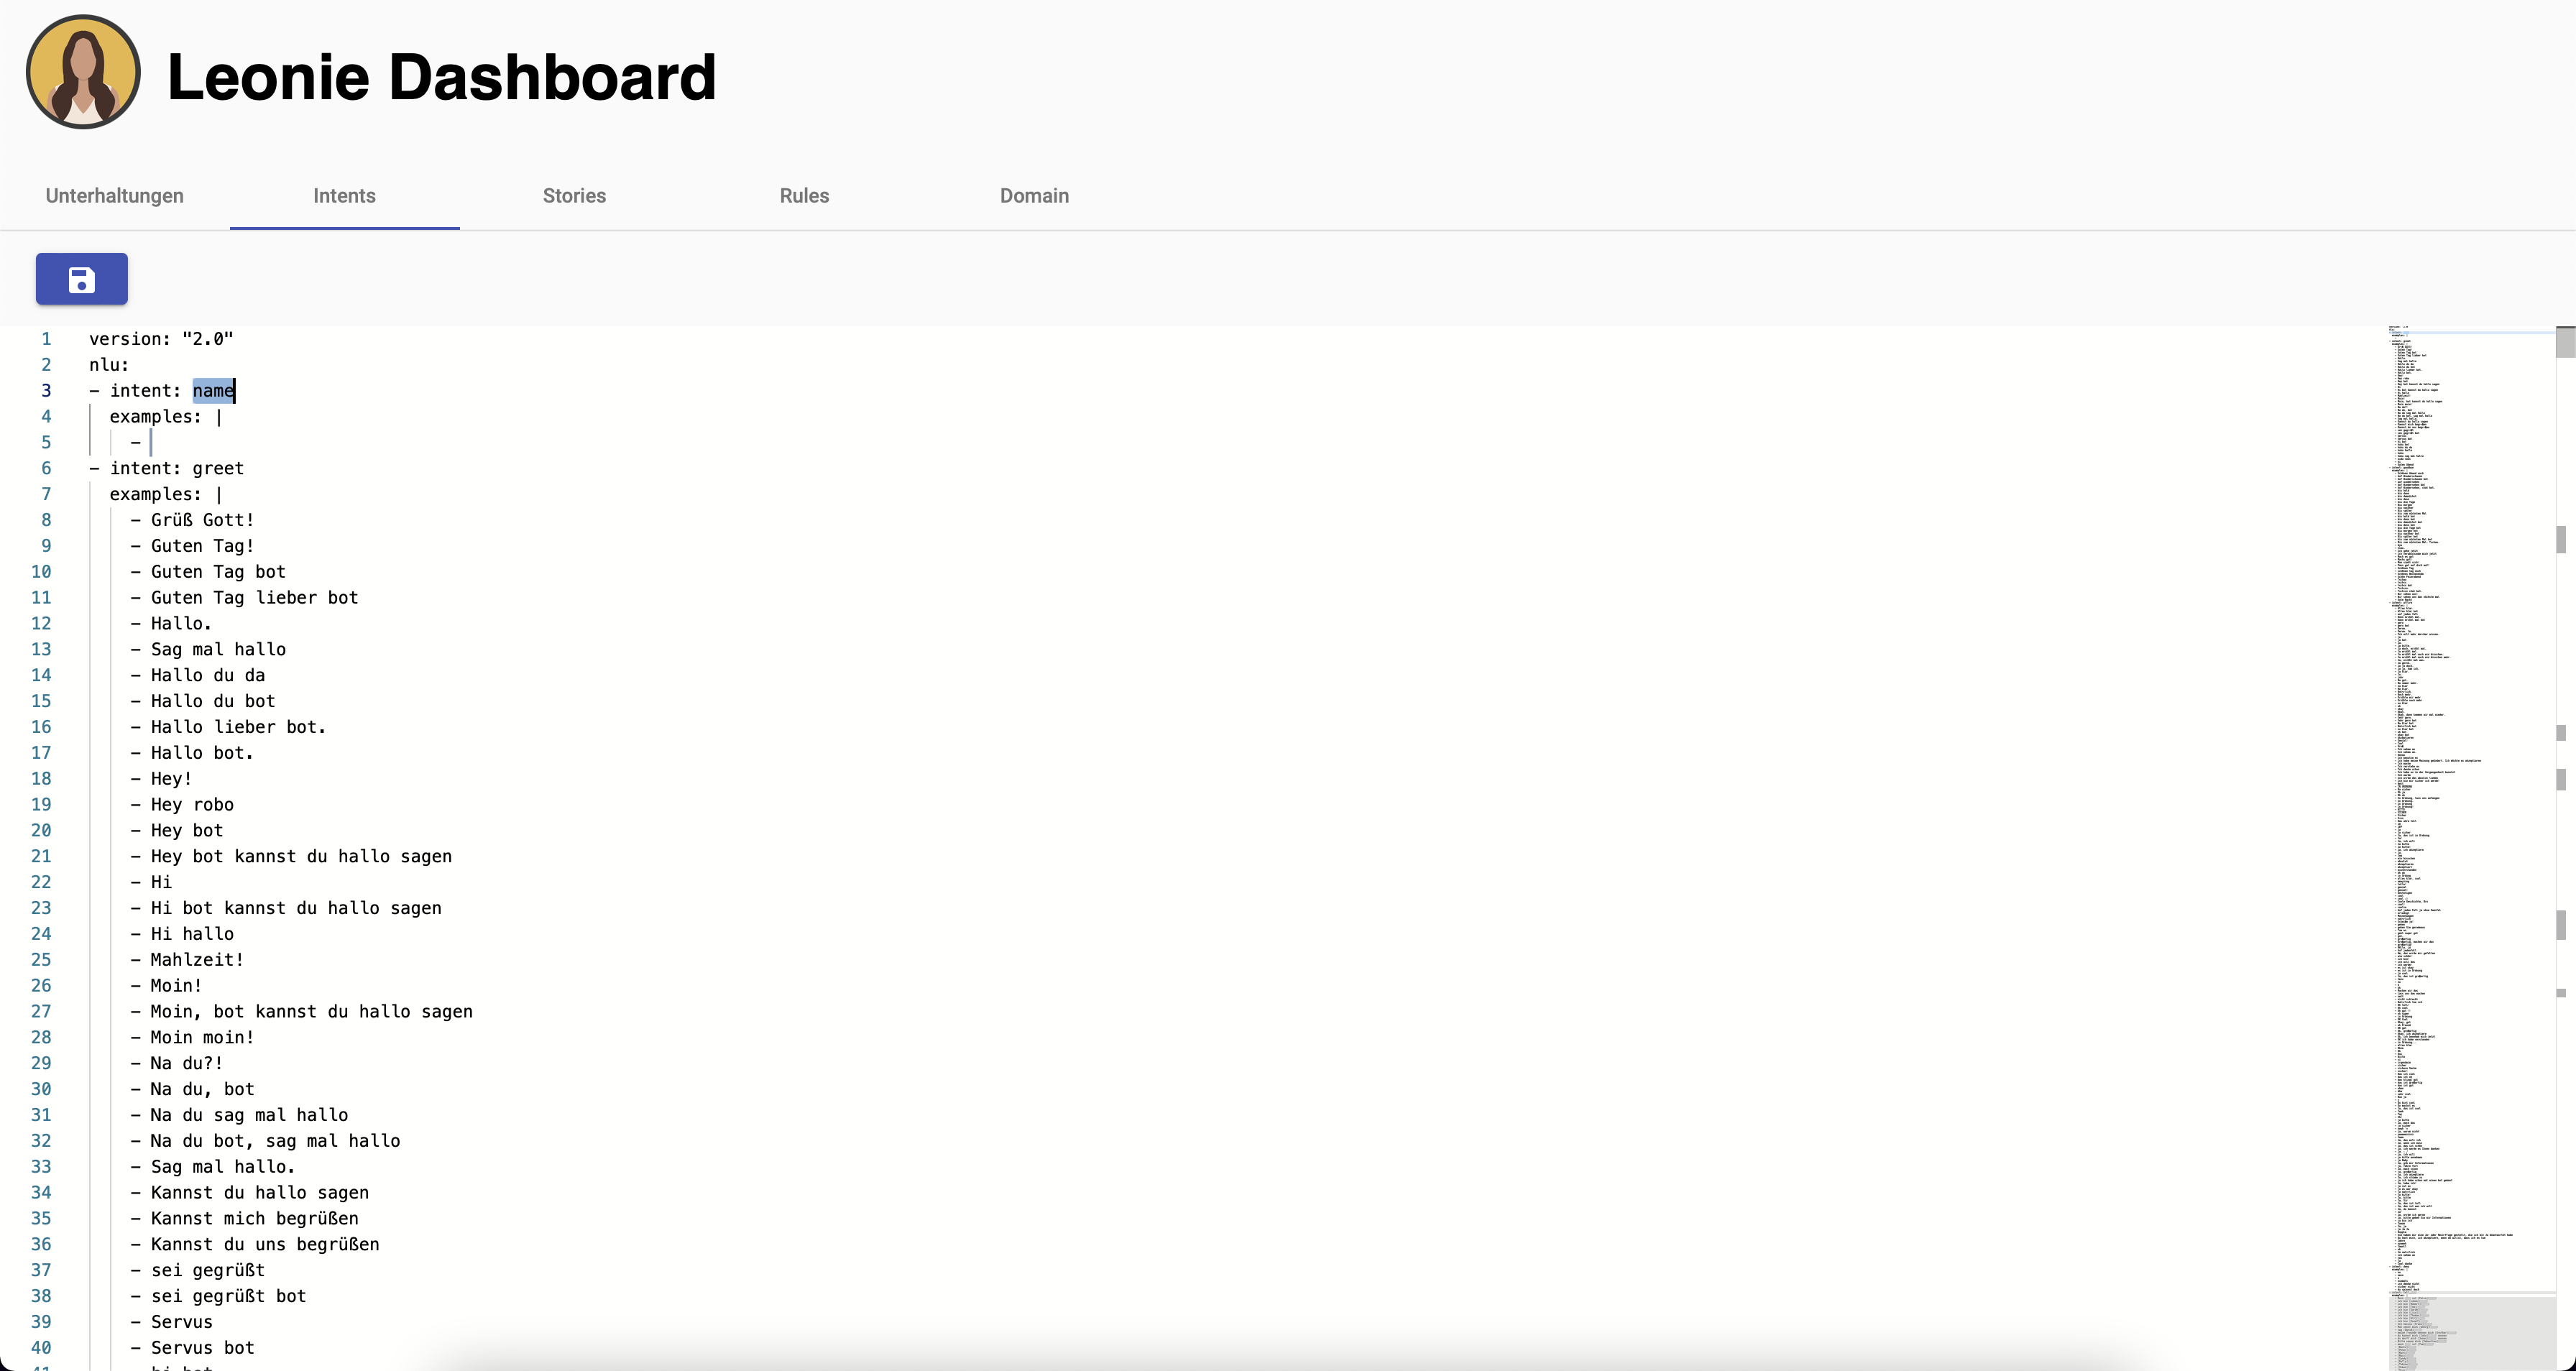
\includegraphics[scale=0.2]{pics/dashboardSuggestionMade}
    \caption{Vorschlag benutzt}
    \label{fig:impl:dashboardCodeSuggestionMade}
\end{figure}



\section{Einbindung in Wordpress}
\subsection{Angular Elements}
''Webkomponenten sind eine Gruppe von Web-Technologien, die es ermöglichen, benutzerdefinierte, wiederverwendbare HTML Elemente zu erstellen, deren Funktionalität gekapselt ist und damit vollständig getrennt von anderem Code.''\cite{webcomponents}

Um unsre Chatkomponente auf die Wordpress Seite zu bringen, entschieden wir uns dazu die Komponente mithilfe von Angular Elements als WebKomponente zu exportieren um somit eine einfache einbindung auf die Schulhomepage zu ermöglichen.

\section{GitHub Actions}

Die Praxische Arbeit besteht aus sehr vielen einzelen Projekten, mit verschiedenen Funktionen, doch bei vielen der GitHub Projekte haben wir mithilfe von GitHub Actions unser Deployment automatisiert.

% TODO
\subsection{Backend}

Unser Backend wird mithilfe von GitHub Actions automatisiert gebaut der Workflow baut das .jar file und dieses wird dann über SSH auf unsre VM geladen.

\subsection{Fronteend}
Die Chat Seite sowie das Dashboard werden mithilfe von GitHub Actions automatisiert gebaut und auf GH Pages gepublished
